%%%%%%%%%%%%%%%%%%%%%%%%%%%%%%%%%%%%%%%%%
% University/School Laboratory Report
% LaTeX Template
% Version 3.1 (25/3/14)
%
% This template has been downloaded from:
% http://www.LaTeXTemplates.com
%
% Original author:
% Linux and Unix Users Group at Virginia Tech Wiki 
% (https://vtluug.org/wiki/Example_LaTeX_chem_lab_report)
%
% License:
% CC BY-NC-SA 3.0 (http://creativecommons.org/licenses/by-nc-sa/3.0/)
%
%%%%%%%%%%%%%%%%%%%%%%%%%%%%%%%%%%%%%%%%%

%----------------------------------------------------------------------------------------
%	PACKAGES AND DOCUMENT CONFIGURATIONS
%----------------------------------------------------------------------------------------

\documentclass[11pt,a4paper]{article}

\usepackage[version=3]{mhchem} % Package for chemical equation typesetting
\usepackage{siunitx} % Provides the \SI{}{} and \si{} command for typesetting SI units
\usepackage{graphicx} % Required for the inclusion of images
\usepackage{natbib} % Required to change bibliography style to APA
\usepackage{amsmath} % Required for some math elements 

\usepackage{listings} 
\usepackage{xcolor} 

\definecolor{mygray}{rgb}{0.4,0.4,0.4}
\definecolor{myorange}{rgb}{1.0,0.4,0}
%http://tex.stackexchange.com/questions/144503/why-does-a-space-destroy-my-keywords-in-listingspackage

\lstset{
 language=C,
basicstyle=\footnotesize\sffamily\color{black},
commentstyle=\color{mygray},
frame=single,
numbers=left,
numbersep=5pt,
numberstyle=\tiny\color{mygray},
keywordstyle=\color{green!70!blue},
showspaces=false,
showstringspaces=false,
stringstyle=\color{myorange},
tabsize=2,  
  morekeywords={
    omp,
    parallel,
    for,    
  }
  alsoother={\#},
  otherkeywords={\#pragma,\#define,\#ifdef,\#endif,\#else},
}

% Fall mal eigene margins definiert werden müssen
%\usepackage{geometry}
% \geometry{
% a4paper,
% total={170mm,257mm},
% left=20mm,
% top=20mm,
% }
% 
\setlength\parindent{0pt} % Removes all indentation from paragraphs

\renewcommand{\labelenumi}{\alph{enumi}.} % Make numbering in the enumerate environment by letter rather than number (e.g. section 6)

%\usepackage{times} % Uncomment to use the Times New Roman font

%----------------------------------------------------------------------------------------
%	DOCUMENT INFORMATION
%----------------------------------------------------------------------------------------

\title{CPA Lab-Report \\ Lab 2 Prime Numbers} % Title

\author{Simon \textsc{Birrer}, Dominic \textsc{Sch\"urmann}} % Author name

\date{\today} % Date for the report

\begin{document}

\maketitle % Insert the title, author and date

\begin{center}
\begin{tabular}{l r}
Date Performed: & October 27, 2015 \\ % Date the experiment was performed
Students: & Simon Birrer \\ % Partner names
& Dominic Sch\"urmann \\
Instructor: & Francisco Javier Piris Ruano % Instructor/supervisor
\end{tabular}
\end{center}

\bigskip

\tableofcontents

\pagebreak

\section{Biggest prime storable in 8 bytes}

The Source for the solution is in the file \textit{primo\textunderscore  grande.c}. In the figure \ref{code_primogrande} you will see the changes applied to function primo of the original code.


\begin{figure}[h]
\label{code_primogrande}
\begin{lstlisting}
   int numberOfThreads;
   int offset;
   #ifdef _OPENMP
   #pragma omp parallel
   numberOfThreads = omp_get_num_threads();
   offset = 2 * numberOfThreads;
   #else
   numberOfThreads = 1;
   offset = 2;
   #endif
    
    #pragma omp parallel private(i)
    {
      #ifdef _OPENMP
      int threadIndex =  omp_get_thread_num();
      int startIndex = (2 * threadIndex) + 3;
      #else
      int startIndex = 3;
      #endif
      for (i = startIndex; p && i <= s; i += offset)
        if (n % i == 0) p = 0;          
    }
\end{lstlisting} 
\caption{code changes primo grande}
\end{figure}


\subsection{Compiling without OpenMP}

To use the program in both ways, either with or without OpenMP , we used the preproccessor directives. Now the compiler decides upon the arguments if the code will use OpenMP or not for the passages where OpenMP function calls will happen.\\

This can be seen in figure \ref{code_primogrande} in lines 3-10 and 14-19.

\pagebreak
\subsection{Time measurement of parallelized version}

In figure \ref{ex12execution} are the measured times of executing the program with different numbers of threads using kahan.\\

\begin{figure}[h]
\centering
  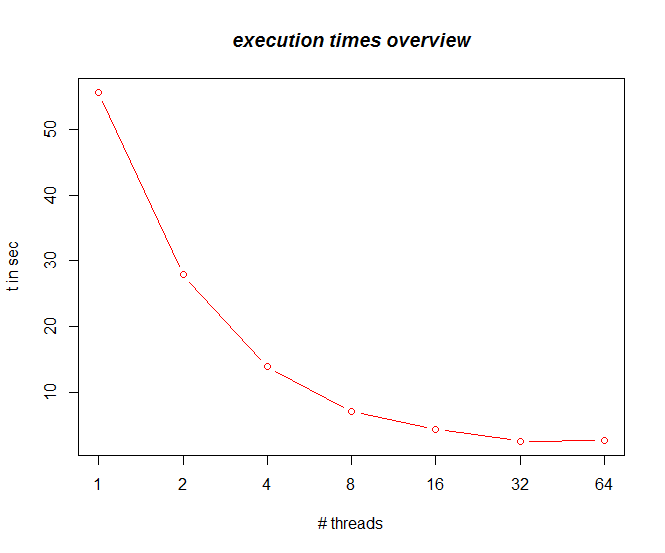
\includegraphics[scale=0.35]{statistics/Ex12ResultGraph.png}
	\caption{execution times for exercise 1.2}
	\label{ex12execution}
\end{figure}


Since a node of kahan has 32 cores, the execution with 32 threads was the fastest. In addition the performance decreases if the number of threads will be increased. This is shown in figure \ref{ex12execution} and the overhead is even more visible in figure \ref{ex12speedUp} .
As a result of this, the best speedup will be achieved with one thread for each processor.

\begin{figure}[h]
\centering
  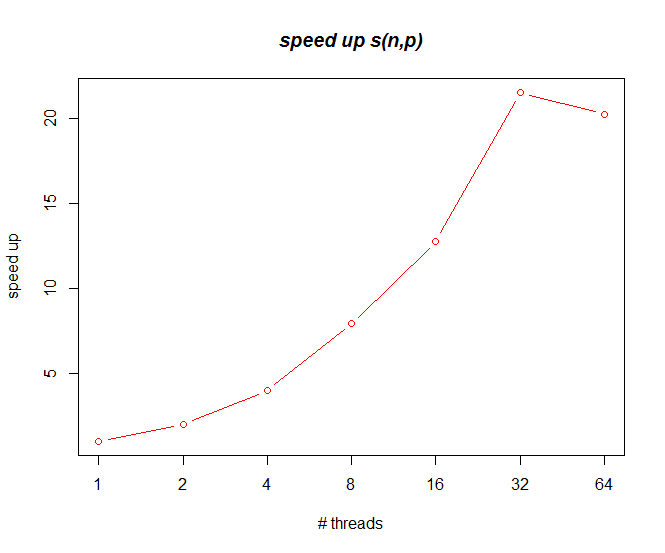
\includegraphics[scale=0.35]{statistics/Ex12SpeedUpGraph.png}
	\caption{speed up for exercise 1.2}
	\label{ex12speedUp}
\end{figure}



\pagebreak

\section{Count primes in a range}

TODO: rewrite!

The Source for the solution of exercise \ref{ex21} is in the file
 \textit{primo\textunderscore numeros\textunderscore 1.c} and
 for exercise \ref{ex22} in file \textit{primo\textunderscore numeros\textunderscore 2.c} \\
 
In all code examples, where a time measurement was needed, following code was used to measure the time in seconds:
 
\begin{figure}[h]
\label{code_timemeasurement}
\begin{lstlisting}
  #ifdef _OPENMP
  double t1 = omp_get_wtime();
  #endif  
  
  //code for algorithm here
  
  #ifdef _OPENMP
  double t2 = omp_get_wtime();
  printf("looptime: %f seconds \n", t2-t1);
  #endif
\end{lstlisting} 
\caption{execution time measurement}
\end{figure} 
 

\subsection{Measurement sequential execution}

To measure the sequential time for the 
\textit{primo\textunderscore numeros\textunderscore .c} code, we compiled the code with OpenMP. To achieve a sequential execution we defined the environment variable
\textit{OMP\textunderscore NUM\textunderscore THREADS = 1}. \\
The sequential execution took 289.24 seconds.


\subsection{Measurement parallel most inner loop}

Based on the exercise a measurement for the most inner loop does not make much sense, because it is really inefficient. Every execution without an if clause in the pragma omp definiton was terminated because of the walltime exceeding.

\subsection{Measurement parallel most outer loop}

The most efficient way to speedup the given exercise code is by parallelize the most outer loop. The following code changes where made to achieve this:

\begin{figure}[h]
\label{code_mostouterloop}
\begin{lstlisting}
  int numberOfThreads;
  #pragma omp parallel
  numberOfThreads = omp_get_num_threads();
  n = 2; /* Por el 1 y el 2 */
  #pragma omp parallel for reduction(+:n) schedule(runtime)
  for (i = 3; i <= N; i += 2){
      if (primo(i))
      {
         n++;
      }
  }
\end{lstlisting} 
\caption{parallelization of the most outer loop}
\end{figure} 

The environment variable was set to 32 Threads to achieve the most biggest speedup.\\

\subsubsection{scheduling distribution}

We checked the execution time for the same code with different scheduling distributions. Therefore we changed the environment variable \textit{OMP\textunderscore SCHEDULE}

\begin{figure}[h]
\centering
\label{table_scheduledistribution}
\begin{tabular}{| l | l | l | l |}
    \hline
    schedule type & chunk size & execution time in [s]\\ 
    \hline
	static & 0 & 17.58 \\
	\hline
	static & 1 & 13.58 \\
    \hline
	dynamic & 0 & 14.18 \\
    \hline
    dynamic & 1 & 14.23 \\
    \hline
    dynamic & 2 & 13.52 \\
    \hline
\end{tabular}
\caption{Measurement result for different schedule distribution}
\end{figure}

\subsection{Exercise 1 without reduction clause}
\label{ex21}

\begin{figure}[h]
\label{code_withoutreduction}
\begin{lstlisting}
  int numberOfThreads;
  #pragma omp parallel
  numberOfThreads = omp_get_num_threads();
  n = 2; /* Por el 1 y el 2 */
  #pragma omp parallel for schedule(runtime)
  for (i = 3; i <= N; i += 2){
      if (primo(i))
      {
         #pragma omp atomic
         n++;
      }
  }
\end{lstlisting} 
\caption{parallelization without reduction}
\end{figure}


\subsection{Exercise 2 printing workload}
\label{ex22}

\pagebreak

\section{appendix}

\subsection{measurements of exercise 1}
\begin{table}[h]
\centering

\label{measuresEx1}
\begin{tabular}{@{}l||l|l|l|l|l|l|l|@{}}
number or threads & 1      & 2      & 4      & 8     & 16    & 32    & 64    \\
\hline	
time in seconds   & 55.571 & 27.850 & 13.931 & 7.019 & 4.349 & 2.580 & 2.741
\end{tabular}
\caption{execution time}
\end{table}

TODO include formula for speed up and speed up table

\listoffigures

\listoftables

%----------------------------------------------------------------------------------------
%	BIBLIOGRAPHY
%----------------------------------------------------------------------------------------

\bibliographystyle{apalike}

\bibliography{sample}

%----------------------------------------------------------------------------------------


\end{document}